\documentclass[a4paper, 12pt, colorlinks=true, linkcolor=black, urlcolor=blue, citecolor=blue, hidelinks]{article}
\usepackage{xcolor}
\usepackage[a4paper, total={6in, 8in}]{geometry}
\usepackage[a-1b]{pdfx}
\usepackage[italian]{babel}
\usepackage{comment}
\usepackage{graphicx}
\usepackage{geometry}
\geometry{
 a4paper,
 total={170mm,257mm},
 left=20mm,
 top=20mm,
 }
\usepackage{csquotes}
\usepackage{svg}
\usepackage{array}
\usepackage{float}
\usepackage{caption}
\usepackage{booktabs}
\usepackage{setspace}
\setstretch{1.5}
\setlength{\parindent}{20pt}
\usepackage[backend=biber, style=numeric, sorting=none]{biblatex}
\usepackage{tocloft} % Add this
\setcounter{tocdepth}{3} % Add this (before \tableofcontents)

\begin{document}
\pagenumbering{roman}


\begin{titlepage} 
      \begin{center}
            \thispagestyle{empty}
            
\includegraphics[width=12.5cm]{Resources/UNIPD_logo.png}
            \begin{spacing}{2.0}
                \Large{DIPARTIMENTO DI MATEMATICA\\LAUREA TRIENNALE IN INFORMATICA}
            \end{spacing}
            \bigskip
            \begin{spacing}{2.0}

                \large{\textbf{PROGETTO DI BASI}}
                \par\rule{\textwidth}{0.5pt}
                \Huge{\textbf{Basi di Dati per la Gestione di un Sistema di Spedizioni}}
                \par\rule{\textwidth}{0.5pt}
                \bigskip
                \bigskip
                \Large{Lorenzo Soligo 2101057, Pietro Bassi 2137999}
            \end{spacing}
      \end{center}
\end{titlepage}
\tableofcontents
\newpage
\pagenumbering{arabic}
\setcounter{page}{1}

\section{Abstract}
Questo lavoro sviluppa una base di dati progettata per gestire in modo strutturato e
coerente le informazioni relative a pacchi, ai clienti, ai corrieri, alle filiali delle aziende trasportatrici . L’obiettivo principale è fornire un sistema che monitori il trasporto di un pacco, attraverso tutti gli step di consegna, gestendone i relativi dati, garantendo un accesso organizzato e facilitando la loro analisi.
Nel contesto della gestione della spedizione di pacchi, la base di dati proposta distingue tra pacchi bundle (come aggregatore di pacchi per un singolo ordine), pacchi assicurati (dotati di tipologie diverse di assicurazione) e pacchi regalo (dotati di una dedica e incartamento non presente nelle altre tipologie). Attributi comuni sono però quelli legati alla tipologia di pacco, costo, dimensioni, date di ordine e di arrivo e un Identificativo.\\ 
Il sistema di Tracking lega all'Identificativo del pacco una DataOra come chiave in modo da costruire uno storico degli aggiornamenti di Status e Posizione per ogni pacco che manterrà come informazione l'ultimo aggiornamento del Tracking. \\Questa base di dati è progettata per garantire un’archiviazione efficiente e strutturata delle informazioni, migliorando il recupero e l’analisi dei dati. L’organizzazione sistematica delle informazioni contribuisce a un utilizzo più efficace delle risorse, ottimizzando la gestione delle strutture di tracking e supportando i processi decisionali.

\newpage
\section{Analisi dei Requisiti}
Questa sezione riassume i requisiti a cui deve sottostare la base di dati.\\
\textbf{Pacco}. Ogni Pacco è identificato da un codice alfanumerico univoco e contiene le seguenti
informazioni:\\
\begin{itemize}
    \setlength{\itemindent}{+.5in}
    \item \textbf{Id} univoco per l'identificazione di un Pacco
    \item \textbf{Tipologia} di prodotto/pacco spedito \footnotesize{(per esempio: elettronica, sanitario, gastronomia ...)}
    \item \normalsize{\textbf{Dimensioni}}
    \item \textbf{Costo}
    \item \textbf{DataOrdine} relativa alla creazione dell'ordine
    \item \textbf{DataPrevista} relativa alla prevista 

\end{itemize}

I pacchi possono essere in: Bundle, Pacchi Assicurati e Pacchi Regalo.\\
\textbf{Bundle}. Oltre alle informazioni generali, per i bundle
\begin{itemize}
    \setlength{\itemindent}{+.5in}
    
    \item 
\end{itemize}
IDEA:: la relazione bundle pacco diventa tabella, bundle infatti legherà ad un codice speciale, gli \textbf{Id} dei pacchi che quel bando comprende.\\
\textbf{Pacchi Assicurati}. Oltre alle informazioni generali, per i Pacchi assicurati si aggiunge:
\begin{itemize}
    \setlength{\itemindent}{+.5in}
    \item \textbf{Tipo Assicurazione} tra una scelta limitata di tipologie:
        \begin{itemize}
            \setlength{\itemindent}{+.5in}
            \item Reso in 30 giorni
            \item Garanzia per un Anno
            \item Garanzia per 3 Anni
        \end{itemize}
\end{itemize}

\textbf{Pacchi Regalo}. Oltre alle informazioni generali, per i Pacchi Regalo si aggiunge:
\begin{itemize}
    \setlength{\itemindent}{+.5in}
    \item \textbf{Tipo Incarto} tra una scelta limitata di tipologie:
        \begin{itemize}
            \setlength{\itemindent}{+.5in}
            \item Carta regalo
            \item Sacchetto in tela
            \item Scatola Speciale
        \end{itemize}
    \item \textbf{Dedica}
\end{itemize}

\textbf{Cliente}. Ogni Cliente è identificato da una email, come nelle registrazioni ai siti (si è preferito questo rispetto a un parametro Id aggiuntivo) e contiene le seguenti
informazioni:
\begin{itemize}
    \setlength{\itemindent}{+.5in}
    \item \textbf{Email} univoco per l'identificazione di un cliente
    \item \textbf{Nome} e un \textbf{Cognome}
    \item \textbf{Indirizzo} necessario per la spedizione
    \item \normalsize{\textbf{Telefono}} presente o meno
\end{itemize}

\textbf{Corriere}. Ogni Corriere è identificato da un C.F. che lo identifica come lavoratore e contiene le seguenti informazioni:
\begin{itemize}
    \setlength{\itemindent}{+.5in}
    \item \textbf{CF} univoco per l'identificazione di un Corriere
    \item \textbf{Agenzia} per cui lavora
    \item \textbf{Grado}, inteso come una sorta di ranking o gerarchia \footnotesize{(ispirato da Death Stranding by  Hideo Kojima)}
    \item \normalsize{\textbf{Mezzo}} di consegna 
    \item \normalsize{\textbf{Disponibilità}} a fare nuove consegne o meno
    \item \textbf{PacchiAttivi} ovvero il numero tutti i pacchi associati ad un corriere e non in stato \textit{"Consegnato"}
\end{itemize}


\textbf{Filiale}. Ogni Filiale è identificata da un Nome e una città che lo identificano come sede e contiene le seguenti informazioni:
\begin{itemize}
    \setlength{\itemindent}{+.5in}
    \item \textbf{Nome} e \textbf{Città} univoco per l'identificazione di una filiale \footnotesize{(ispirato ai locker Amazon per il ritiro e a Death Stranding)}
    \item \textbf{Indirizzo} precisa la posizione
    \item \textbf{Tipo} distingue tra:
     \begin{itemize}
            \setlength{\itemindent}{+.5in}
            \item Locker
            \item Punto di Controllo
            \item Magazzino
        \end{itemize}
\end{itemize}

\textbf{Tracking}. Ogni Tracking rappresenta lo storico di un pacco. È identificato dal \textbf{Id} del pacco tracciato e dalla \textbf{DataOra} del tracciamento che lo identifica come storico e contiene le seguenti informazioni:
\begin{itemize}
    \setlength{\itemindent}{+.5in}
    \item \textbf{Id} e \textbf{DataOra} univoco per l'identificazione di un Tracking System
    \item \textbf{Note} per specifiche considerazioni, se necessarie
    \item \textbf{Status} distingue tra:
     \begin{itemize}
            \setlength{\itemindent}{+.5in}
            \item Consegnato
            \item In Consegna
            \item Spedito
            \item Autorizzato
            \item Fase di Controllo
        \end{itemize}
\end{itemize}



\begin{figure}[H]
\centering
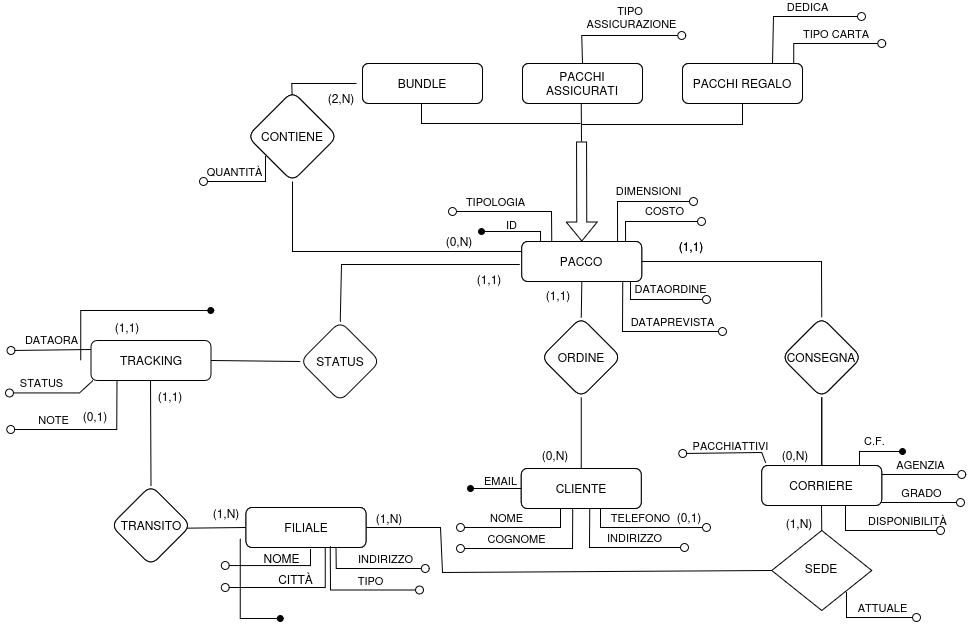
\includegraphics[width=1.0\textwidth]{Resources/ER.png}
\caption{Diagramma ER della Base di Dati relativa al sistema di spedizioni}
\label{ER}
\end{figure}
– 
\section{Progettazione Concettuale}

Il Diagramma \ref{ER} riassume i requisiti della sezione 2.\\ Esistono 3 tipi di Pacchi: Bundle, Pacchi Assicurati, Pacchi Regalo.
Bundle risulta particolarmente singolare in quanto implementa una struttura ricorsiva. Per natura infatti un bundle è un insieme di elementi, nel caso specifico di pacchi.\\
Necessita particolari attenzioni anche l'entità `Tracking`. Questa rappresenta sostanzialmente uno storico degli aggiornamenti nel tempo delle informazioni di status e posizione di un pacco. Per ogni DataOra di un determinato Pacco viene infatti associato uno Status, una Posizione presso le filiali dell'azienda di spedizione e eventualmente anche una Nota come descritto sopra. L'entità pacco invece manterrà solo l'ultimo degli aggiornamenti di stato, ovvero quello che nell'insieme dei Tracking avrà il suo Id e il valore maggiore di DataOra.\\
La relazione Sede indica rispettivamente la sede di appartenza di un Corriere, specificando se si tratti della sede attuale o passata attraverso l'attributo booleano ATTUALE. Si tratta quindi di una relazione molti a molti che rappresenta lo storico delle sedi a cui è appartenuto un Corriere. Trattandosi di una relazione N a N non è comparsa nell'Analisi dei requisiti e verrà gestita con la creazione di una tabella SEDE.

\section{Progettazione Logica}

In questa sezione viene illustrato il processo di “traduzione” dello schema concettuale in uno schema logico, con l’obiettivo di rappresentare i dati in modo preciso
ed efficiente. Il primo passo consiste nell’analizzare le eventuali ridondanze nel modello, al fine di ottimizzare la struttura complessiva. Successivamente, si procede
con l’eliminazione delle due generalizzazioni. Infine, viene presentato il diagramma
ristrutturato, con una descrizione delle modifiche apportate.

\subsection{Analisi Ridondanze}

L'attributo PACCHIATTIVI in CORRIERE esprime il numero di pacchi non ancora consegnati che sono associati a ogni corriere. Ciò corrisponde a una ridondanza dato che si tratta di un numero calcolabile contando, per ogni corriere, il numero di pacchi il cui corrispettivo TRACKING ha l'attributo STATUS diverso da \textit{"Consegnato"}.
Questo attributo viene modificato ogni volta che un pacco viene consegnato o associato al corriere. Viene invece visualizzato ogni mezz'ora per monitorare l'operato di ogni corriere. Il numero di pacchi associati al giorno per un corriere è in media di 120\footnote{\href{https://www.dire.it/26-02-2019/301816-video-a-milano-la-rabbia-dei-corrieri-di-amazon-quattro-minuti-a-consegna-troppo-pochi/}{Fonte di riferimento per i "120 pacchi al giorno". 2019}}.\\
Questo si riassume nelle due seguenti operazioni:
\begin{itemize}
    \item \textbf{Operazione 1 (120 volte al giorno)}: memorizza il numero di pacchi non consegnati associati ad ogni corriere.
    \item \textbf{Operazione 2 (48 volte al giorno)}: visualizza il numero di pacchi non consegnati associati ad ogni corriere
\end{itemize}


\begin{table}[H]
    \centering
    \begin{tabular}{p{2.5cm} p{4cm} p{5cm} p{3cm}}
    \toprule
    \textbf{Entità} & \textbf{Descrizione} & \textbf{Attributi} & \textbf{Identificatore} \\
    \midrule
    Filiale         & Filiale di un'azienda di spedizione & Nome, Città, Tipo, Indirizzo & Nome, Città \\
    
    Tracking        & Storico del Tracking di un pacco & DataOra, IdPacco, Status, Note, NomeCheckPoint, CittàCheckPoint & IdPacco, DataOra \\
    
    Pacco           & Elemento spedito & Id, Tipologia, Dimensioni, Costo, DataOrdine, DataSpedizione & Id \\
    
    Pacchi Assicurati & Pacco Assicurato & TipoAssicurazione & — \\
    
    Pacchi Regalo   & Pacco Regalo & Dedica, TipoCarta & — \\
    
    Cliente         & Proprietario del Pacco & Email, Nome, Cognome, Indirizzo, Telefono & Email \\
    
    Corriere        & Addetto alla spedizione di un pacco & C.F., Grado, Disponibilità, PacchiAttivi & C.F. \\
    \bottomrule
    \end{tabular}
    \caption{Tabella delle Entità}
    \label{tab:entità}
\end{table}

\begin{table}[H]
    \centering
    \begin{tabular}{clcc}
    \toprule
    \textbf{Relazione} & \textbf{Descrizione} & \textbf{Componente} & \textbf{Attributi}  \\ [0.5ex] 
    \midrule
        Sede & Sede di un Corriere & Corriere, Filiale & Attuale\\
        Transito & Posizione Pacco & Tracking, Filiale & \\
        Status & Informazioni sul tracciamento del pacco & Pacco, Tracking & \\
        Contiene & Composizione dei Bundle & Pacco,Bundle & Quantità \\
        Ordine & Ordine di un pacco di un cliente & Cliente, Pacco &  \\
        Consegna & Consegna di un pacco da parte di un Corriere & Corriere, Pacco & \\
        \bottomrule
    \end{tabular}
    \caption{Tabella delle Relazioni}
    \label{tab:relzioni}
\end{table}



Assumendo i seguenti volumi nella base di dati:

\begin{table}[H]
\centering
\begin{tabular}{lcc}
\toprule
\textbf{Concetto} & \textbf{Costrutto} & \textbf{Volume} \\ [0.5ex]
\midrule
    Corriere & E & 1000 \\
    Tracking & E & 120 000 \\
    Pacco & E & 120 000 \\
    Consegna & R & 120 000 \\
    Status & R & 120 000 \\
\bottomrule
    \end{tabular}
    \caption{Tabella dei Volume}
\end{table}


la seguente analisi serve per stabilire se sia utile o meno tenere l’attributo ridondante
PACCHIATTIVI in CORRIERE.

\textbf{Con Ridondanza:} Analizziamo prima il costo totale con ridondanza.\\
\textbf{Operazione 1:} 

\begin{table}[H]
\centering
\begin{tabular} {lllll}
    \toprule
    \textbf{Concetto} & \textbf{Costrutto} & \textbf{Accessi} & \textbf{Tipo} & \textbf{Accessi al giorno}\\ [0.5ex]
    \midrule
        Tracking & E & 1 & S & 120\\
        Pacco & E & 1 & S & 120\\
        Status & R & 1 & S & 120\\
        Corriere & E & 1 & S & 120\\
    \bottomrule
\end{tabular}
\caption{Tabella dei Volume}
\end{table}


\textbf{Operazione 2:}\\
\begin{table}[H]
\centering
\begin{tabular} {lllll}
    \toprule
    \textbf{Concetto} & \textbf{Costrutto} & \textbf{Accessi} & \textbf{Tipo} & \textbf{Accessi al giorno}\\ [0.5ex]
    \midrule
        Corriere & E & 1 & L & 48\\
    \bottomrule
\end{tabular}
\caption{Tabella dei Volume}
\end{table}

Assumendo costo doppio per gli accessi in scrittura rispetto a quelli in lettura, il costo totale con ridondanza è:
Costo totale con ridondanza = 120*4*2+48*1= 1080+48=1128

\textbf{Senza Ridondanza:} Analizziamo prima il costo totale senza ridondanza.
\begin{itemize}
    \item \textbf{Operazione 1:} 
     
        \begin{table}[H]
        \centering
        \begin{tabular} {lllll}
        \toprule
        \textbf{Concetto} & \textbf{Costrutto} & \textbf{Accessi} & \textbf{Tipo} & \textbf{Accessi al giorno}\\ [0.5ex]
        \midrule
            Tracking & E & 1 & S & 120\\
            Pacco & E & 1 & S & 120\\
            Status & R & 1 & S & 120\\ 
        \bottomrule
           \end{tabular}
            \caption{Tabella dei Volume}
    \end{table}

    \item \textbf{Operazione 2(Con circa 120 000/1000=120 pacchi consegnati al giorno):}
        \begin{table}[ht]
        \centering
        \begin{tabular} {lcccc}
        \toprule
        \textbf{Concetto} & \textbf{Costrutto} & \textbf{Accessi} & \textbf{Tipo} & \textbf{Accessi al giorno}\\ [0.5ex]
        \midrule
            Corriere & E & 1 & L & x48\\
            Pacco & E & 120 & L & x48\\
            Consegna & R & 120 & L & x48\\ 
            \bottomrule
           \end{tabular}
            \caption{Tabella dei Volume}
    \end{table}

\end{itemize}
Assumendo costo doppio per gli accessi in scrittura rispetto a quelli in lettura, il costo totale senza ridondanza è:
Costo totale senza ridondanza = 120*3*2+48*1+120*48*2= 720+48+11520=12288

\textbf{Conclusione:} Il costo totale con ridondanza è 1128, mentre il costo totale senza ridondanza è 12288.\\
L'analisi suggerisce dunque di mantenere l'attributo ridondante PACCHIATTIVI in CORRIERE, in quanto il costo totale con ridondanza è significativamente inferiore rispetto al costo totale senza ridondanza, rendendo così gli accessi ottimizati.\\
Inoltre, l'attributo ridondante PACCHIATTIVI in CORRIERE è utile per monitorare l'operato di ogni corriere e per ottimizzare le operazioni di consegna.
L'attributo pacchi attivi, per essere implementato correttamente in SQL, avrebbe bisogno di alcuni vincoli che consentano un aggiornamento automatico dei suoi valori.\\
Per implementare tale vincoli i CHECK non sono sufficienti, sarebbero necessarie delle nozioni (come quella di Trigger) che non sono state affrontate durante il corso.\\
Nello schema logico, l'attributo PACCHIATTIVI in CORRIERE è stato mantenuto e manualmente i suoi valori sono stati resi coerenti con gli altri presenti. Non viene però garantito il vincolo che sarebbe concettualmente necessario in quanto non implementabile con gli strumenti attuali.





\subsection{Eliminazione delle Generalizzazioni}

Le generalizzazioni descritte in Sezione 3 vengono eliminate attraverso una ristrutturazione dello schema concettuale, con l’obiettivo di semplificare la successiva implementazione del modello relazionale e ridurre la presenza di valori nulli. Le modifiche
vengono applicate come segue:

\textbf{PACCHI}: La generalizzazione parziale di PACCHI viene rimossa tramite tre operazioni distinte che si occupano delle tre entità figlie, realizzando dunque una soluzione "ibrida".\\
Per PACCHI ASSICURATI e per PACCHI REGALO si è deciso di sostituire la generalizzazione con l'accorpamento delle due entità figlie nel padre. Le due entità figlie verranno dunque eliminate e 
la loro funzione sarà sostituita da degli attributi che saranno attribuiti all'entità padre. 
Questa scelta si giustifica di fronte al basso livello di "profondità" e "annidamento" degli attributi delle entità figlie in questione. Infatti queste entità non hanno relazioni con altre entità che non siano quella padre. 
Ne consegue dunque che l'introduzione di ulteriori attributi nel padre produce una quantità di valori NULL limitata, che non produce un effetto a cascata su ulteriori entità. Infatti in questo caso la presenza di valori NULL negli attributi sostituivi sarà dunque limitata a soli tre attributi.\\
L'entità figlia BUNDLE dispone già di per sé di una relazione con l'entità padre e merita dunque un trattamento differente. Il vincolo originario che un PACCO ASSICURATO, non possa essere anche PACCO REGALO e viceversa verrà quindi mantenuto grazie alla creazione di check che controllano che gli stati dei parametri nel padre siano coerenti: se alcuni specifici di un tipo di pacco sono \textit{not null}, altrispecifici dell'altro tipo dovranno essere \textit{null}.\\
Incorporarla direttamente nella relazione padre renderebbe la sua gestione particolarmente complessa, con la necessità dell'aggiunta di numerosi attributi per mantenere l'insieme delle caratteristiche originali. Questo corrisponderebbe tra l'altro a un numero rilevante di attributi che si troverebbero poi molto spesso a essere messi a NULL (nel caso di un non-BUNDLE). 
Un'altra opzione consisterebbe  nell'aggiungere un'altra relazione tra BUNDLE e PACCHI, riducendo in questo caso il numero di potenziali NULL. In questo caso però si avrebbero però due relazioni e due entità per gestire una struttura che corrisponde a una semplice entità con una relazione ricorsiva con un attributo. Abbiamo dunque deciso di optare per quest'ultima operazione di traduzione che comporta una notevole semplificazione e una gestione efficiente delle risorse disponibili.\\
Sono inoltre necessari due ulteriori controlli del vincolo nella tabella BUNDLE e in TRACKING.In BUNDLE per evitare che un pacco possa contenere se stesso, quindi \textit{IdBUndle} e \textit{IdContenuto} non possono essere uguali.\\
In TRACKING invece è necessario che tutte le \textit{DataOra} siano successive alla \textit{DataOra} di creazione del pacco.\\
Tali controlli non sono stati implementati in SQL, per mancanza di conoscenze necessarie.\\
\begin{figure}[H]
\centering
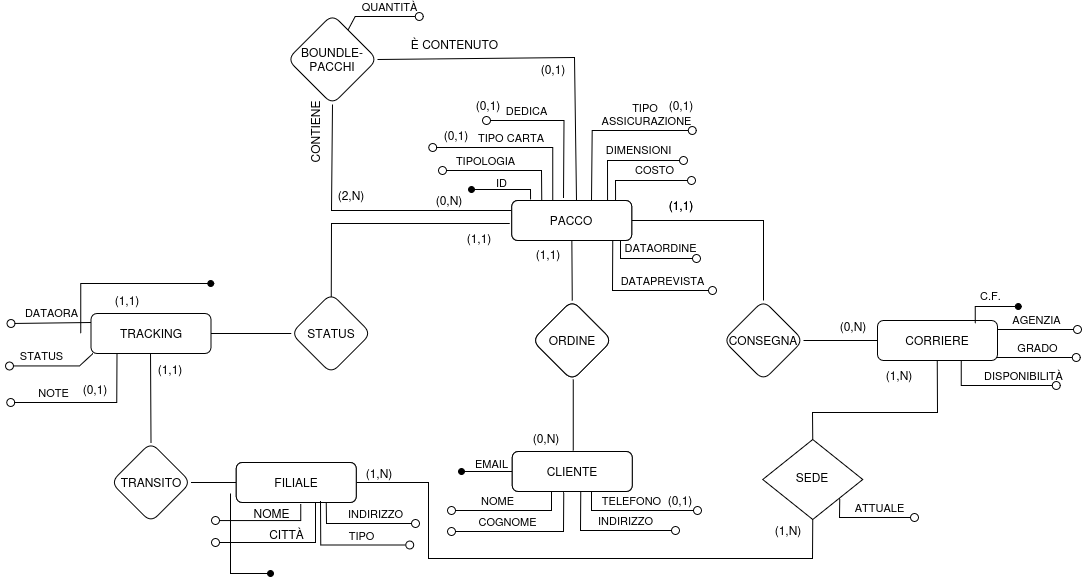
\includegraphics[width=1 \textwidth]{Resources/ML.png}
\caption{Diagramma della Base di Dati dopo l'eliminazione delle Generalizzazioni}
\label{ML}
\end{figure}

\subsection{Schema Relazionale}
Lo schema ristrutturato in Figura \ref{ML} contiene solamente costrutti mappabili in corrispettivi dello schema relazionale detto anche schema logico. Lo schema logico è rappresentato a seguire, dove l'asterisco dopo il nome degli attributi indica quelli che ammettono valori nulli.
\begin{itemize}
    \setlength{\itemindent}{+0in}
    \item \textbf{Pacco}(\underline{ID}, Tipologia, Dimensioni, Costo, DataOraOrdine, DataOraPrevista, Cliente, Corriere, TipoAssicurazione*, Dedica*, TipoCarta*)
        \begin{itemize}
            \setlength{\itemindent}{+.2in}
            \item Pacco.Cliente $\rightarrow$ Cliente.Email 
            \item Pacco.Corriere $\rightarrow$ Corriere.C.F.
        \end{itemize}
    \item \textbf{Bundle-Pacchi}(\underline{IdBundle, IdContenuto}, Quantità)
        \begin{itemize}
            \setlength{\itemindent}{+.2in}
            \item Bundle.IdBundle $\rightarrow$ Pacco.Id 
            \item Bundle.IdContenuto $\rightarrow$ Pacco.Id
        \end{itemize}
        
    \item \textbf{Corriere}(\underline{C.F.}, Agenzia, Grado, Disponibilità, Pacchi Attivi)
    \item \textbf{Filiale}(\underline{Nome, Città}, Tipo, Indirizzo)
    \item \textbf{Tracking}(\underline{IdPacco, DataOra}, Status, Note*, NomeCheckPoint,\\CittàCheckPoint)
        \begin{itemize}
                \setlength{\itemindent}{+.2in}
                \item Tracking.IdPacco $\rightarrow$ Pacco.Id
                \item Tracking.(NomeCheckPoint, CittàCheckPoint) $\rightarrow$ Filiale.(Nome, Città)
        \end{itemize}
    \item \textbf{Cliente}(\underline{Email}, Nome, Cognome, Indirizzo, Telefono*)
     \item \textbf{Sede}(\underline{Corriere, SedeNome, SedeCittà}, Attuale)
        \begin{itemize}
            \setlength{\itemindent}{+.2in}
            \item Sede.Corriere $\rightarrow$ Corriere.C.F.
            \item Sede.(SedeNome, SedeCittà) $\rightarrow$ Filiale.(Nome, Città)
        \end{itemize}
     
\end{itemize}

\section{Implementazione in PostgreSQL e Definizione
delle Query}

\subsection{Definizione delle Query}

1. \textbf{QUERY 1} Media del costo dei pacchi di un corriere di un certo grado che sono passati per una filiale di un certo tipo
  \begin{figure}[H]
\centering
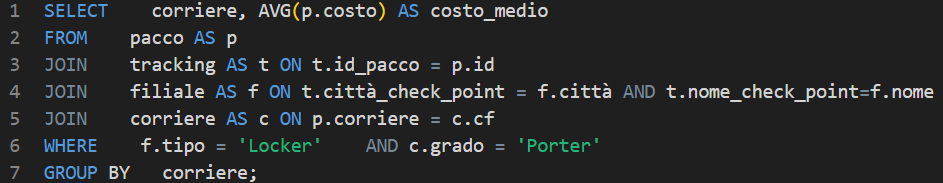
\includegraphics[width=0.8 \textwidth]{Resources/QUERY1.png}
\label{Q1}
\end{figure}
2. \textbf{QUERY 2} Numero pacchi per bundle con garanzia 3 anni
\begin{figure}[H]
\centering
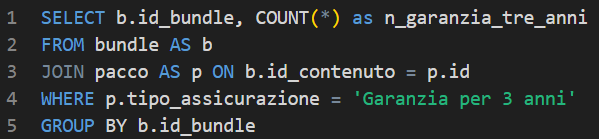
\includegraphics[width=0.6 \textwidth]{Resources/QUERY2.png}
\label{Q2}
\end{figure}
3. \textbf{QUERY 3} Corrieri che hanno un tempo di consegna medio dei loro pacchi superiore al tempo medio di consegna di un pacco:
\begin{figure}[H]
\centering
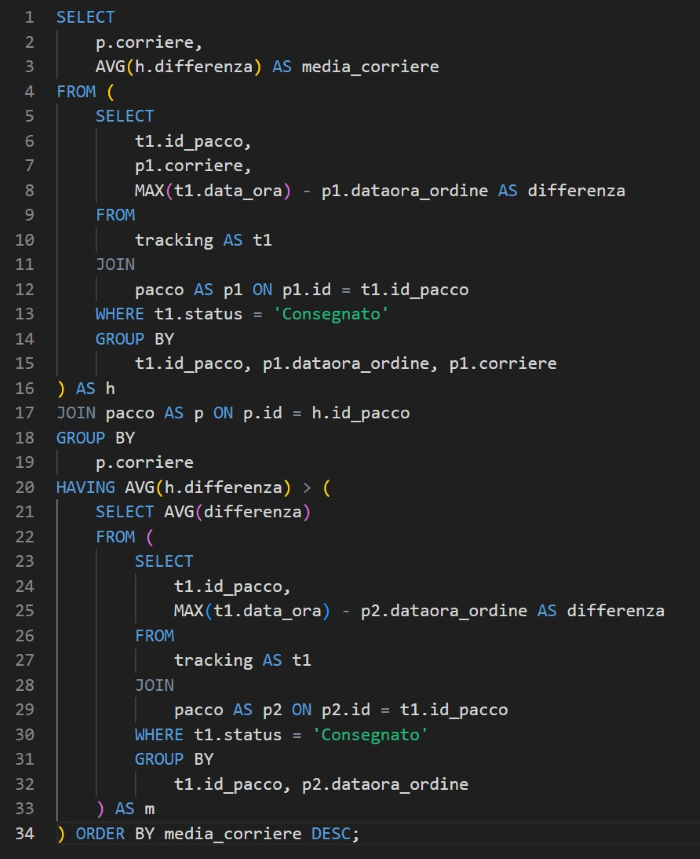
\includegraphics[width=0.6 \textwidth]{Resources/QUERY3.png}
\label{Q3}
\end{figure}
4. \textbf{QUERY 4} Corrieri con bundle con pacchi con garanzia a 3 anni e costo maggiore di 300
\begin{figure}[H]
\centering
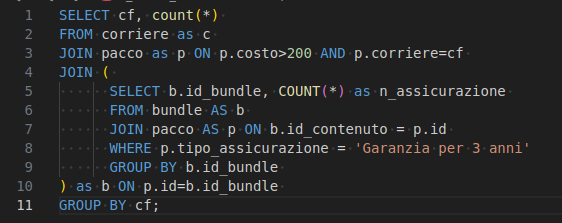
\includegraphics[width=0.7 \textwidth]{Resources/QUERY4.png}
\label{Q4}
\end{figure} 
5. \textbf{QUERY 5} Ultimo aggiornamento del tracking di un pacco
\begin{figure}[H]
\centering
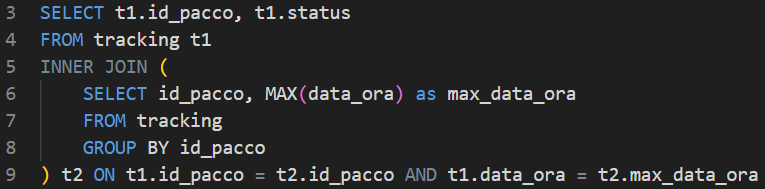
\includegraphics[width=0.7 \textwidth]{Resources/QUERY5.png}
\label{Q5}
\end{figure}

\subsection{Creazione degli Indici} 

Supponendo di voler ottimizzare la query num 5, si deve considerare:

\begin{itemize}
  \item Condizione del JOIN: \texttt{t.id\_pacco = p.id}
  \item Condizione del JOIN: \texttt{t.città\_check\_point = f.città AND t.nome\_check\_point = f.nome}
  \item Condizione del JOIN: \texttt{p.corriere = c.cf}
  \item Condizione del WHERE: \texttt{ f.tipo = 'Locker'AND c.grado = 'Porter'}
  \item GROUP BY sulle colonne: \texttt{corriere}
\end{itemize}


\noindent Per il punto 1 è opportuno creare due indici hash su entrambe le colonne del join:
\begin{figure}[H]
\centering
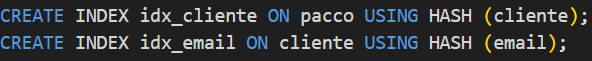
\includegraphics[width=0.8 \textwidth]{Resources/INDEX1.png}
\label{I1}
\end{figure}

\noindent Per il punto 2 è opportuno creare quattro indici hash per tutte le condizioni del join:
\begin{figure}[H]
\centering
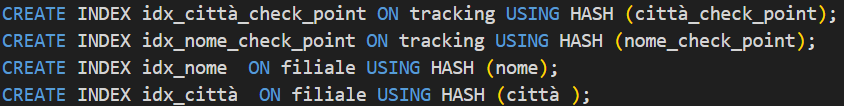
\includegraphics[width=0.8 \textwidth]{Resources/INDEX2.png}
\label{I2}
\end{figure}

\noindent Per il punto 3 è opportuno creare due indici hash su entrambe le colonne del join:

\begin{figure}[H]
\centering
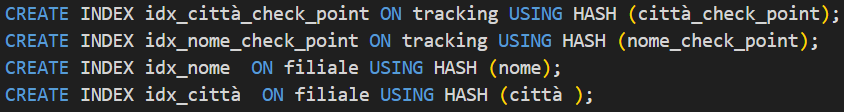
\includegraphics[width=0.7 \textwidth]{Resources/INDEX3.png}
\label{I3}
\end{figure}

\noindent Per il punto 4 è opportuno creare due indici per i due attributi rispetto a cui il WHERE valuta la sua condizione:

\begin{figure}[H]
\centering
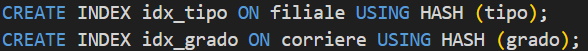
\includegraphics[width=0.7 \textwidth]{Resources/INDEX4.png}
\label{I4}
\end{figure}

\noindent Il punto 5 è un GROUP BY e potrebbe quindi essere ottimizzato tramite il seguente indice B+Tree:
 
\begin{figure}[H]
\centering
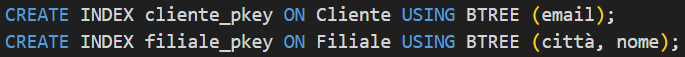
\includegraphics[width=0.8 \textwidth]{Resources/INDEX5.png}
\label{I5}
\end{figure}  

\noindent Visto che non si tratta di un attributo che è chiave primaria di una entità POSTGRE non ha già creato l'indice B+TREE corrispondente ed è necessario crearlo manualmente.
\section{Applicazione Software}
\begin{comment}
\begin{lstlisting}[caption={Example C Code}]
... definizioni e inclusioni necessarie ...

const char *STATUS[] = {
    "Consegnato",
    "In Consegna",
    "Spedito",
    "Autorizzato",
    "Fase di Controllo"};

... altri enum per evitare errori di battitura ...

... funzioni per la connessione al database ...

void printResult(int rows, int cols, PGresult *res)
{
    for (int i = 0; i < rows; i++)
    {
        for (int j = 0; j < cols; j++)
        {
            printf("%s\t\t", PQgetvalue(res, i, j));
        }
        printf("\n");
    }
}

int main(int argc, char **argv)
{
    .
    .
    .
    int end = 0;
    while (end != 1)
    {
        printf("Premi invio per continuare...\n");
        getchar();

        int scelta;
        printf("Che query vuoi eseguire?\n A tua disposizione abbiamo queste 5 opzioni:\n");
        printf("\t1. Media del costo dei pacchi di un corriere di un certo grado che sono passati per una filiale di un certo tipo\n\t2. Numero pacchi per bundle con un determinato tipo di assicurazione\n\t3. Corrieri con tempi di consegna maggiori alla media\n\t4. Corrieri con bundle con pacchi assicurati o regalo e costo specifici\n\t5. Status attuale dei pacchi\n");
        printf("Qual'è la tua scelta? (1-5): ");
        scanf("%d", &scelta);
        while (scelta < 1 || scelta > 5)
        {
            printf("\tHai scelto... molto MALE!\n\tTrovo insopportabile la sua mancanza di Input corretto\n");
            printf("Le scelte sono 5, riprova: ");
            scanf("%d", &scelta);
        }
        printf("\tHai scelto molto bene!  (cit)\n\n");
        PGresult *res;

        if (scelta == 1)
        {
            const char *query1 = "SELECT corriere, AVG(p.costo) AS costo_medio "
                                 "FROM pacco AS p "
                                 "JOIN tracking AS t ON t.id_pacco = p.id "
                                 "JOIN filiale AS f ON t.città_check_point = f.città AND t.nome_check_point=f.nome "
                                 "JOIN corriere AS c ON p.corriere = c.cf "
                                 "WHERE f.tipo = $1 AND c.grado = $2 "
                                 "GROUP BY corriere;";
            res = PQprepare(conn, "query1", query1, 2, NULL);
            if (PQresultStatus(res) != PGRES_COMMAND_OK)
            {
                fprintf(stderr, "Prepare failed: %s", PQerrorMessage(conn));
                PQclear(res);
            }
            PQclear(res);

            int grado;
            int tipo_filiale;
            printf("Scegli il Tipo di Filiale. Le opzioni sono:\n");
            for (int i = 0; i < 3; i++)
            {
                printf("\t%d. %s\n", i + 1, TIPO_FILIALE[i]);
            }
            printf("Quale tipo vuoi? (1-3): ");
            scanf("%d", &tipo_filiale);
            while (tipo_filiale < 1 || tipo_filiale > 3)
            {
                printf("\tHai scelto... molto MALE!\n\tTrovo insopportabile la sua mancanza di Input corretto\n");
                printf("Quale grado vuoi? (1-4): ");
                scanf("%d", &tipo_filiale);
            }

            printf("Scegli il Grado del Corriere. Le opzioni sono:\n");
            for (int i = 0; i < 4; i++)
            {
                printf("\t%d. %s\n", i + 1, GRADO_CORRIERE[i]);
            }
            printf("Quale grado vuoi? (1-4): ");
            scanf("%d", &grado);
            while (grado < 1 || grado > 4)
            {
                printf("\tHai scelto... molto MALE!\n\tTrovo insopportabile la sua mancanza di Input corretto\n");
                printf("Quale grado vuoi? (1-4): ");
                scanf("%d", &grado);
            }

            const char *paramValues[2] = {
                TIPO_FILIALE[tipo_filiale - 1],
                GRADO_CORRIERE[grado - 1]};

            res = PQexecPrepared(conn, "query1", 2, paramValues, NULL, NULL, 0);
            checkResults(res, conn);

            // Stampa i risultati
            int rows = PQntuples(res);
            int cols = PQnfields(res);

            printf("\n\t\tMedia del costo dei pacchi di un corriere %s che sono passati per una filiale %s:\n", GRADO_CORRIERE[grado - 1], TIPO_FILIALE[tipo_filiale - 1]);
            printf("ID Corriere\t\t\tCosto Medio\n");
            printf("-----------\t\t\t-----------\n");
            printResult(rows, cols, res);
            PQclear(res);
        }

        if (scelta == 2)
        {
            const char *query2 = "SELECT b.id_bundle, COUNT(*) as n_garanzia_tre_anni "
                                 "FROM bundle AS b "
                                 "JOIN pacco AS p ON b.id_contenuto = p.id "
                                 "WHERE p.tipo_assicurazione = $1 "
                                 "GROUP BY b.id_bundle";
            res = PQprepare(conn, "query2", query2, 1, NULL);

            int assicurazione;
            printf("Scegli il tipo di assicurazione. Le opzioni sono:\n");
            for (int i = 0; i < 3; i++)
            {
                printf("\t%d. %s\n", i + 1, TIPO_ASSICURAZIONE[i]);
            }
            printf("Quale tipo vuoi? (1-3): ");
            scanf("%d", &assicurazione);
            while (assicurazione < 1 || assicurazione > 3)
            {
                printf("\tHai scelto... molto MALE!\n\tTrovo insopportabile la sua mancanza di Input corretto\n");
                printf("Quale grado vuoi? (1-3): ");
                scanf("%d", &assicurazione);
            }

            const char *paramValue = TIPO_ASSICURAZIONE[assicurazione - 1];
            res = PQexecPrepared(conn, "query2", 1, &paramValue, NULL, NULL, 0);
            checkResults(res, conn);

            // Stampa i risultati
            int rows = PQntuples(res);
            int cols = PQnfields(res);

            printf("\nNumero pacchi per bundle con %s:\n", TIPO_ASSICURAZIONE[assicurazione - 1]);
            printf("ID Bundle\t\t\tNumero pacchi Assicurati\n");
            printf("---------\t\t\t------------------------\n");
            printResult(rows, cols, res);
            PQclear(res);
        }

        if (scelta == 3)
        {
            const char *query3 = "SELECT p.corriere, AVG(h.differenza) AS media_corriere "
                                 "FROM ( "
                                 "    SELECT t1.id_pacco, p1.corriere, MAX(t1.data_ora) - p1.dataora_ordine AS differenza "
                                 "    FROM "
                                 "        tracking AS t1 "
                                 "    JOIN pacco AS p1 ON p1.id = t1.id_pacco "
                                 "    WHERE t1.status = 'Consegnato' "
                                 "    GROUP BY t1.id_pacco, p1.dataora_ordine, p1.corriere "
                                 ") AS h "
                                 "JOIN pacco AS p ON p.id = h.id_pacco "
                                 "GROUP BY p.corriere "
                                 "HAVING AVG(h.differenza) > ( "
                                 "    SELECT AVG(differenza) "
                                 "    FROM ( "
                                 "        SELECT t1.id_pacco, MAX(t1.data_ora) - p2.dataora_ordine AS differenza "
                                 "        FROM tracking AS t1 "
                                 "        JOIN pacco AS p2 ON p2.id = t1.id_pacco "
                                 "        WHERE t1.status = 'Consegnato' "
                                 "        GROUP BY t1.id_pacco, p2.dataora_ordine "
                                 "    ) AS m "
                                 ") "
                                 "ORDER BY media_corriere DESC;";
            PGresult *res = PQexec(conn, query3);
            checkResults(res, conn);

            // Stampa i risultati
            int rows = PQntuples(res);
            int cols = PQnfields(res);

            printf("\nCorrieri più lenti del tempo medio di consegna:\n");
            printf("ID Corriere\t\t\tTempo di consegna medio\n");
            printf("-----------\t\t\t-----------------------\n");

            printResult(rows, cols, res);
            PQclear(res);
        }

        if (scelta == 4)
        {
            int costo;
            printf("Scegli il costo per il filtraggio dei risultati: ");
            scanf("%d", &costo);
            char costo_str[12];
            snprintf(costo_str, sizeof(costo_str), "%d", costo);

            int filtro;
            printf("Vuoi filtrare per pacchi assicurati o regalo?    (0=assicurati, 1=regalo): ");
            scanf("%d", &filtro);
            while (filtro < 0 || filtro > 1)
            {
                printf("\n Input non valido, riprova: ");
                printf("Vuoi filtrare per pacchi assicurati o regalo?    (0=assicurati, 1=regalo): ");
                scanf("%d", &filtro);
            }
            if (filtro == 0)
            {
                const char *query4 = "SELECT cf, count(*) "
                                     "FROM corriere as c "
                                     "JOIN pacco as p ON p.costo>$1 AND p.corriere=cf "
                                     "JOIN ( "
                                     "      SELECT b.id_bundle, COUNT(*) as n_garanzia_tre_anni "
                                     "      FROM bundle AS b "
                                     "      JOIN pacco AS p ON b.id_contenuto = p.id "
                                     "      WHERE p.tipo_assicurazione = $2"
                                     "      GROUP BY b.id_bundle "
                                     ") as b ON p.id=b.id_bundle "
                                     "GROUP BY cf";
                res = PQprepare(conn, "query4", query4, 2, NULL);
                int assicurazione;

                printf("Scegli il tipo di assicurazione. Le opzioni sono:\n");
                for (int i = 0; i < 3; i++)
                {
                    printf("\t%d. %s\n", i + 1, TIPO_ASSICURAZIONE[i]);
                }
                printf("Quale tipo vuoi? (1-3): ");
                scanf("%d", &assicurazione);
                while (assicurazione < 1 || assicurazione > 3)
                {
                    printf("\tHai scelto... molto MALE!\n\tTrovo insopportabile la sua mancanza di Input corretto\n");
                    printf("Quale grado vuoi? (1-3): ");
                    scanf("%d", &assicurazione);
                }

                const char *paramValues[2] = {
                    costo_str,
                    TIPO_ASSICURAZIONE[assicurazione - 1]};
                res = PQexecPrepared(conn, "query4", 2, paramValues, NULL, NULL, 0);
            }
            else
            {
                int caso;
                printf("Cosa vuoi dalla query:\n\t1. Solo tipo carta\n\t2. Solo dedica\n\t3. Entrambi\n Cosa preferisci? (1-3): ");
                scanf("%d", &caso);
                while (caso < 1 || caso > 3)
                {
                    printf("\n Input non valido, riprova: ");
                    printf("Cosa vuoi dalla query:\n\t1. Solo tipo carta\n\t2. Solo dedica\n\t3. Entrambi\n Cosa preferisci? (1-3): ");
                    scanf("%d", &filtro);
                }

                if (caso == 1)
                {
                    const char *query4a = "SELECT cf, count(*) "
                                          "FROM corriere as c "
                                          "JOIN pacco as p ON p.costo>$1 AND p.corriere=cf "
                                          "JOIN ( "
                                          "      SELECT b.id_bundle, COUNT(*) as n_garanzia_tre_anni "
                                          "      FROM bundle AS b "
                                          "      JOIN pacco AS p ON b.id_contenuto = p.id "
                                          "      WHERE p.tipo_carta = $2"
                                          "      GROUP BY b.id_bundle "
                                          ") as b ON p.id=b.id_bundle "
                                          "GROUP BY cf";
                    res = PQprepare(conn, "query4a", query4a, 2, NULL);
                    int assicurazione;

                    int carta;
                    printf("Scegli il tipo di carta. Le opzioni sono:\n");
                    for (int i = 0; i < 3; i++)
                    {
                        printf("\t%d. %s\n", i + 1, TIPO_CARTA[i]);
                    }
                    printf("Quale tipo vuoi? (1-3): ");
                    scanf("%d", &carta);
                    while (carta < 0 || carta > 3)
                    {
                        printf("\tHai scelto... molto MALE!\n\tTrovo insopportabile la sua mancanza di Input corretto\n");
                        printf("Quale carta vuoi? (1-3): ");
                        scanf("%d", &carta);
                    }

                    const char *paramValues[2] = {
                        costo_str,
                        TIPO_CARTA[carta - 1]};
                    res = PQexecPrepared(conn, "query4a", 2, paramValues, NULL, NULL, 0);
                }

                else if (caso == 2)
                {
                    const char *query4b = "SELECT cf, count(*) "
                                          "FROM corriere as c "
                                          "JOIN pacco as p ON p.costo>$1 AND p.corriere=cf "
                                          "JOIN ( "
                                          "      SELECT b.id_bundle, COUNT(*) as n_garanzia_tre_anni "
                                          "      FROM bundle AS b "
                                          "      JOIN pacco AS p ON b.id_contenuto = p.id "
                                          "      WHERE p.dedica = $2"
                                          "      GROUP BY b.id_bundle "
                                          ") as b ON p.id=b.id_bundle "
                                          "GROUP BY cf";
                    res = PQprepare(conn, "query4b", query4b, 2, NULL);

                    char dedica[100];
                    printf("Inserisci la dedica: ");
                    scanf("%99s", dedica);

                    const char *paramValues[2] = {
                        costo_str,
                        dedica};
                    res = PQexecPrepared(conn, "query4b", 2, paramValues, NULL, NULL, 0);
                }

                else
                {
                    const char *query4c = "SELECT cf, count(*) "
                                          "FROM corriere as c "
                                          "JOIN pacco as p ON p.costo>$1 AND p.corriere=cf "
                                          "JOIN ( "
                                          "      SELECT b.id_bundle, COUNT(*) as n_garanzia_tre_anni "
                                          "      FROM bundle AS b "
                                          "      JOIN pacco AS p ON b.id_contenuto = p.id "
                                          "      WHERE p.tipo_carta = $2 AND p.dedica = $3"
                                          "      GROUP BY b.id_bundle "
                                          ") as b ON p.id=b.id_bundle "
                                          "GROUP BY cf";
                    res = PQprepare(conn, "query4c", query4c, 3, NULL);

                    int carta;
                    printf("Scegli il tipo di carta. Le opzioni sono:\n");
                    for (int i = 0; i < 3; i++)
                    {
                        printf("\t%d. %s\n", i + 1, TIPO_CARTA[i]);
                    }
                    printf("Quale tipo vuoi? (1-3): ");
                    scanf("%d", &carta);
                    while (carta < 0 || carta > 3)
                    {
                        printf("\tHai scelto... molto MALE!\n\tTrovo insopportabile la sua mancanza di Input corretto\n");
                        printf("Quale carta vuoi? (1-3): ");
                        scanf("%d", &carta);
                    }

                    char dedica[100];
                    printf("Inserisci la dedica: ");
                    scanf("%99s", dedica);

                    const char *paramValues[3] = {
                        costo_str,
                        TIPO_CARTA[carta - 1],
                        dedica};
                    res = PQexecPrepared(conn, "query4c", 3, paramValues, NULL, NULL, 0);
                }
            }

            checkResults(res, conn);

            // Stampa i risultati
            int rows = PQntuples(res);
            int cols = PQnfields(res);
            printf("Corriere\t\t\tNumero pacchi\n");
            printf("--------\t\t\t------\n");

            // printf("\nCorrieri con bundle con pacchi con %s e costo maggiore di %d", TIPO_ASSICURAZIONE[assicurazione - 1], costo);
            printResult(rows, cols, res);
            PQclear(res);
        }

        if (scelta == 5)
        {
            const char *query5 = "SELECT t1.id_pacco, t1.status "
                                    "FROM tracking t1 "
                                    "INNER JOIN ("
                                    "    SELECT id_pacco, MAX(data_ora) as max_data_ora "
                                    "    FROM tracking "
                                    "    GROUP BY id_pacco"
                                    ") t2 ON t1.id_pacco = t2.id_pacco AND t1.data_ora = t2.max_data_ora;";
            PGresult *res = PQexec(conn, query5);
            checkResults(res, conn);

            // Stampa i risultati
            int rows = PQntuples(res);
            int cols = PQnfields(res);

            printf("\nRisultati della vista ultimo_tracking:\n");
            printf("ID Pacco\t\t\tStatus\n");
            printf("--------\t\t\t------\n");

            printResult(rows, cols, res);
            PQclear(res);
        }

        printf("\n\nVuoi continuare? (0=si, 1=no): ");
        scanf("%d", &end);
    }
    printf("Grazie per aver usato il mio programma! Che l'algebra relazionale sia con te\n");
    // Pulizia e chiusura
    PQfinish(conn);

    return 0;
}
\end{lstlisting}
\end{comment}

Il codice code.c permette di connettersi al database PostGres su Supabase, scelto perchè permette di lavorare in condivisione.\\
Una volta effettuata la connessione, il programma permette di eseguire 5 query diverse, a scelta dell'utente.\\
Tre delle 5 query sono state scritte in modo da essere parametrizzate, in modo da evitare SQL injection, questo grazie agli \textit{enum} che restringono la scelta dei parametri a solo quelli possibili.
\begin{itemize}
            \setlength{\itemindent}{+.2in}
            \item Media del costo dei pacchi di un corriere di un certo grado che sono passati per una filiale di un certo tipo
                  Parametrizzabile per il tipo di filiale e grado del corriere.
            \item Numero pacchi per bundle con un determinato tipo di assicurazione
                  Parametrizzabile per il tipo di assicurazione.
            \item Corrieri con tempi di consegna maggiori alla media.
            \item Corrieri con bundle con pacchi assicurati o regalo e costo specifici. 
                Parametrizzabile per tutti i valori \textit{Assicurati e Regalo} e per il Costo.
            \item Status attuale dei pacchi
\end{itemize}

\end{document}